\documentclass[titlepage]{article}
\usepackage{fancyhdr}
\usepackage{datetime}
\usepackage{color}
\usepackage{tikz}
\fancyhf{}

\topmargin=-0.45in
\evensidemargin=0in
\oddsidemargin=0in
\textwidth=6.5in
\textheight=9.0in
\headsep=0.25in

\newcommand{\noteTitle}{\formatdate{31}{1}{2016} --- Notes}
\newcommand{\professor}{Guangzhi Qu}
\newcommand{\class}{CSE 450 Operating Systems}
\newcommand{\classTime}{Monday \& Wednesday 3:30 --- 5:17 pm}
\newcommand{\notesAuthor}{Nicholas Land}

\pagestyle{fancy}
\lhead{\notesAuthor}
\chead{\class}
\rhead{\noteTitle}
\lfoot{}
\cfoot{\thepage}
\rfoot{}
\renewcommand{\headrulewidth}{0.4pt}
\renewcommand{\footrulewidth}{0.4pt}

\title{
  \textmd{\LARGE{\textbf{\noteTitle}}}\\
  \textmd{\Large{\textit{\class}}}\\
  \textmd{\Large{\textit{Professor\ \professor}}}\\
  \textmd{\normalsize{\classTime}}\\
  \vspace{3.5in}
  \textmd{\LARGE{\textbf{\notesAuthor}}}\\
  \date{}
}

\begin{document}
  \maketitle

  \section*{gnuplot}
  We can use gnuplot to generate nice plots for us! \\
    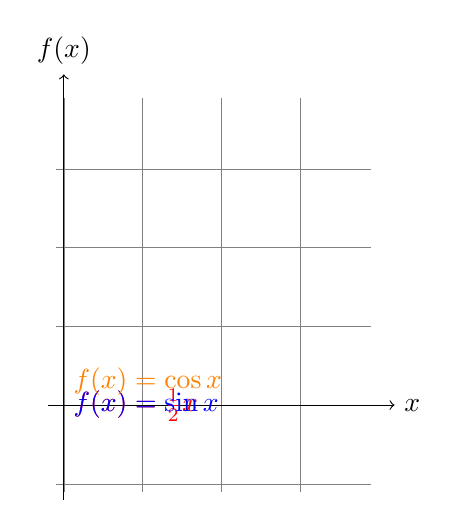
\begin{tikzpicture}[domain=0:4]
      \draw[very thin,color=gray] (-0.1,-1.1) grid (3.9,3.9);
      \draw[->] (-0.2,0) -- (4.2,0) node[right] {$x$};
      \draw[->] (0,-1.2) -- (0,4.2) node[above] {$f(x)$};
      \draw[color=red] plot[id=x] function{0.5*x}
        node[right] {$f(x) =\frac{1}{2}x$};
      \draw[color=blue] plot[id=sin] function{sin(x)}
        node[right] {$f(x) = \sin x$};
      \draw[color=orange] plot[id=cos] function{cos(x)}
        node[above right] {$f(x) = \cos x$};
    \end{tikzpicture}

  \section*{Section 2}

  \section*{Section 3}

\end{document}
